\documentclass[12pt,a4paper]{article}
\usepackage{amsmath,amssymb}
\usepackage{graphicx}
\usepackage{float}
\usepackage{tikz}
\usetikzlibrary{shapes, arrows, positioning}


\usepackage{amsmath,amssymb,mdframed}            % AMS package gives better equation layouts
\setcounter{page}{5}                    % sets first page number to 2
\setlength{\oddsidemargin}{-0.25in}     % set left margin
\setlength{\textwidth}{6.5in}           % set text width
\setlength{\topmargin}{-0.5in}          % controls layout at
\setlength{\headsep}{0.5in}             % top of page
\setlength{\textheight}{9.0in}          % set text length



\makeatletter
\renewcommand{\@oddhead}{\hfill MA3600/Mock}  % sets header
\renewcommand{\@oddfoot}{\hfil \arabic{page} \hfil}    % sets page footer
\makeatother

\renewcommand{\labelenumi}{\arabic{enumi}} % Sets the first level of enumerate to be arabic (normal) numbers
\renewcommand{\labelenumii}{(\alph{enumii})} %Sets the second level of enumerate to be (a), (b), (c), .....
\renewcommand{\labelenumiii}{(\roman{enumiii})} % Sets the third level of enumerate to be (i), (ii), (iii), ....



\begin{document}
\null \vskip1cm
\begin{enumerate}
\setcounter{enumi}{3}

\renewcommand\labelenumi{\bfseries\theenumi.}

\item

    \begin{enumerate}
        \item Provide definitions for the following terms:
            \begin{itemize}
                \item Normal form game.

                ~\hfill{[1]}

                \item Strictly dominated strategy.

                ~\hfill{[1]}

                \item Weakly dominated strategy.

                ~\hfill{[1]}

                \item Best response strategy.

                ~\hfill{[1]}

                \item Nash equilibrium.

                ~\hfill{[1]}
            \end{itemize}

        For the remainder of this question consider the battle of the sexes game:

            \[\begin{pmatrix}
            (1,-1) & (-2,2)\\
            (-3,3) & (1,-1)\\
            \end{pmatrix}\]

        \item By clearly stating the techniques used: obtain all (if any) pure Nash equilibrium.

        ~\hfill{[4]}

        \item Plot the utilities to player 1 (the row player) assuming that the 2nd player (the column player) plays a mixed strategy: $\sigma_2 = (y,1-y)$.

        ~\hfill{[2]}

        \item Plot the utilities to player 2 (the column player) assuming that the 1st player (the row player) plays a mixed strategy: $\sigma_1 = (x,1-x)$.

        ~\hfill{[2]}

        \item Assuming that player 1 plays the mixed strategy $\sigma_1=(x,1-x)$, show that player 1's best response $x^*$ to a mixed strategy $\sigma_2 = (y,1-y)$ is given by:


            \[
            x^*=\begin{cases}
                0,&\text{ if } y < 3/7\\
                1,&\text{ if } y > 3/7\\
                \text{indifferent},&\text{ otherwise }\\
            \end{cases}
            \]

            Similarly show that player 2's best response $y^*$ is given by:

            \[
            y^*=\begin{cases}
                0,&\text{ if } x < 4/7\\
                1,&\text{ if } x > 4/7\\
                \text{indifferent},&\text{ otherwise }\\
            \end{cases}
            \]

        ~\hfill{[4]}

        \item Use the above to obtain all Nash equilibria for the game.

        ~\hfill{[2]}

        \item Confirm this result by stating, proving and using the Equality of Payoffs theorem.

        ~\hfill{[6]}

    \end{enumerate}

\newpage
\item

    \begin{enumerate}

            \item Consider the centipede game shown below:

            \begin{center}
                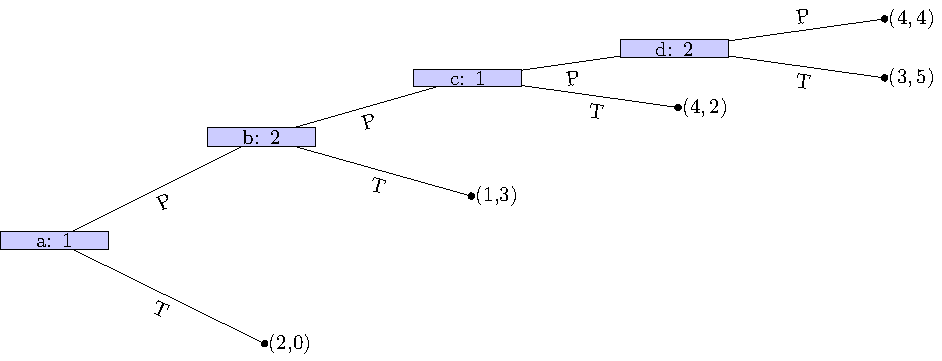
\includegraphics[width=.8\textwidth]{images/mock-img01.pdf}
            \end{center}

            Obtain a subgame perfect Nash equilibrium for this game (you are expected to prove that it is a subgame perfect Nash equilibrium).

            \hfill[11]

            \item Prove the following theorem:

            ``For any finitely repeated game, any sequence of stage Nash profiles gives the outcome of a subgame perfect Nash equilibrium.''

            \hfill[4]

            \item If they exist identify (prove) all subgame perfect Nash equilibrium for the following two games:

                \begin{center}
                    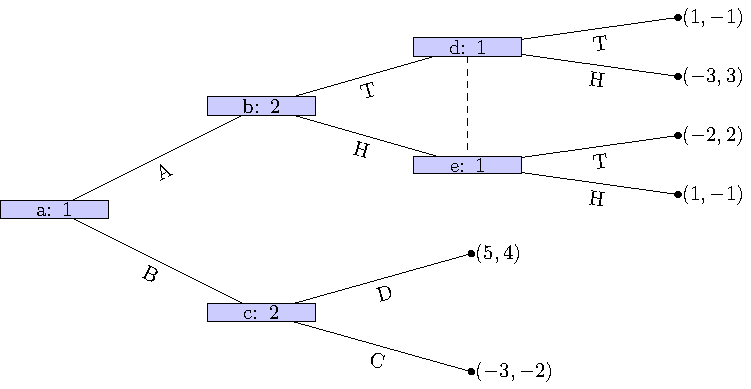
\includegraphics[width=.8\textwidth]{images/mock-img02.pdf}\\
                    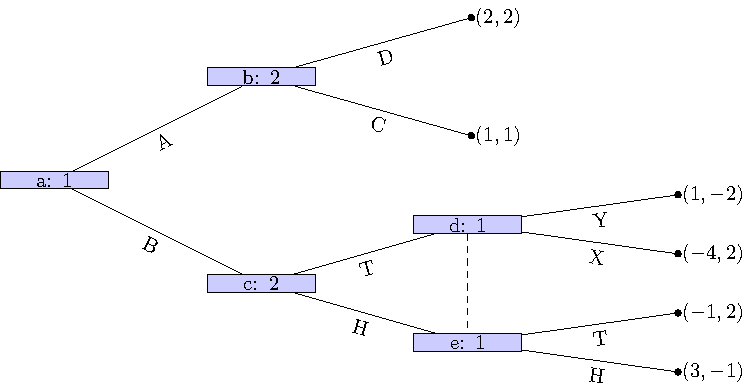
\includegraphics[width=.8\textwidth]{images/mock-img03.pdf}
                \end{center}

            \hfill[10]

    \end{enumerate}

\newpage
\item

    \begin{enumerate}

        \item Define a stochastic game.

        \hfill[4]

        \item Define a Markov strategy.

        \hfill[2]

        \item Give the conditions for Nash equilibrium in a stochastic game.

        \hfill[3]

        \item Obtain the pure strategy Nash equilibria (if it exists) for the following game with \(\delta=.5\):

        \begin{center}
            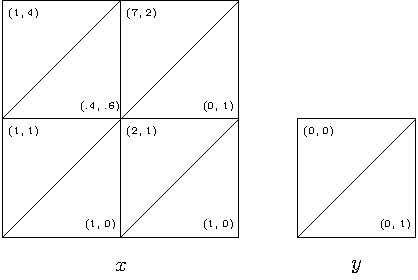
\includegraphics[width=.8\textwidth]{images/mock-img04.pdf}
        \end{center}

        \hfill[16]

    \end{enumerate}
\end{enumerate}


\makeatletter
\renewcommand{\@oddfoot}{\hfil \arabic{page}X \hfil}    % sets last page footer
\makeatother

\end{document}
